\chapter{浮游生物图像分类}

研究浮游生物图像自动分类,既需要了解浮游生物领域的相关知识,也要掌握计算机视觉和机器学习领域的相关理论。本章作为介绍基于多核学习的浮游生物图像分类研究的预备知识章节,首先介绍浮游生物的基础知识,然后对后续实验使用的数据集进行说明,接下来介绍目前分类性能较好的浮游生物图像分类方法,在本章最后介绍评价分类系统性能所采用的评价方法。

\section{浮游生物基本知识介绍}

% 浮游生物介绍,分别介绍浮游植物和动物
浮游生物是指生活在水中运动能力较弱的生物体,它们是许多大型水生生物的食物,包括浮游植物和动物两大类。浮游植物是一种微小的植物,在水中以浮游状态生存,通常是指浮游藻类,包括裸藻门、黄藻门、金藻门、绿藻门、甲藻门、硅藻门、蓝藻门、隐藻门八个门类,目前已知的浮游植物约有4万种。浮游动物是生活在水中的无脊椎动物和脊索动物幼体的总称,其种类繁多,主要的门类有原生动物、浮游幼虫、甲壳纲、毛颚动物、腔肠动物、被囊动物等。

% 浮游生物个体大小
浮游生物通常较小,个体从几微米到几毫米大小不等,按照个体的大小可以将其分为以下几类:小于5微米为超微型浮游生物;5至50微米之间为微型浮游生物;50微米到1毫米之间为小型浮游生物;1至5毫米之间为中型浮游生物;5毫米到10毫米间为大型浮游生物;大于1厘米为巨型浮游生物。通常浮游植物的个体相对浮游动物较小,一般属于微型和小型浮游生物;而浮游动物体型通常较大,主要为中型、大型以及巨型浮游生物。由于大多浮游生物较小,因此必须使用显微镜进行观测。

% 浮游生物形态特征
浮游生物是按照界、门、纲、目、科、属、种的分类学原理进行分类的,从上层的“界”到下层的“种”,越往下层被归为同一个分支的浮游生物之间形态特征越相似。因此在对浮游生物进行分类时,时常会遇到形态特征十分相似的两个不同类别的浮游生物生物,这一特点增加了浮游生物分类识别的难度。例如,图~\ref{fig:changjian}中的浮游生物为长腹剑水蚤属,而图~\ref{fig:beikou}中为杯口水蚤目,这两幅图像中的浮游生物分别属于桡脚类亚纲下的剑水蚤目和杯口水蚤目,但它们的形态特征十分相似,不易区分。
\begin{figure}[h]
  \centering%
  \subcaptionbox{长腹剑水蚤属\label{fig:changjian}}%标题的长度,超过则会换行,如下一个小图。
    {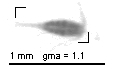
\includegraphics[height=2.5cm]{chart2/changjian}}%
  \hspace{2em}%
  \subcaptionbox{杯口水蚤目\label{fig:beikou}}
      {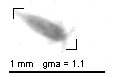
\includegraphics[height=2.5cm]{chart2/beikou}}\\
  \caption{桡脚类亚纲下的两类浮游生物图像}
  \label{fig:raojiao}
\end{figure}


\section{数据集介绍}
\label{sec:dataset}

为了设计一个泛化能力强、适用范围广的浮游生物图像分类系统,本文搜集构建了以下三个不同浮游生物数据集进行实验:一个是由伍兹霍尔海洋研究所(Woods Hole Oceanographic Institution, WHOI)使用FlowCytobot采集的浮游植物数据集;另一个是使用ZooScan系统采集的浮游动物数据集;还有Kaggle竞赛中使用的浮游生物数据集。

\subsection{WHOI采集的数据集}
\label{sec:whoidataset}

在美国的大西洋海岸上有一个综合性海洋科学研究机构——伍兹霍尔海洋研究所,其致力于对海洋中各个领域进行研究。本数据集~\cite{sosik2007automated}是由该机构研究人员使用FlowCytobot采集的2004至2005年间伍兹霍尔港附近的浮游植物图像组成,该数据集一共包括22类浮游植物图像,其例图如图~\ref{fig:whoi}所示。
\begin{figure}[H] % use float package if you want it here
  \centering
  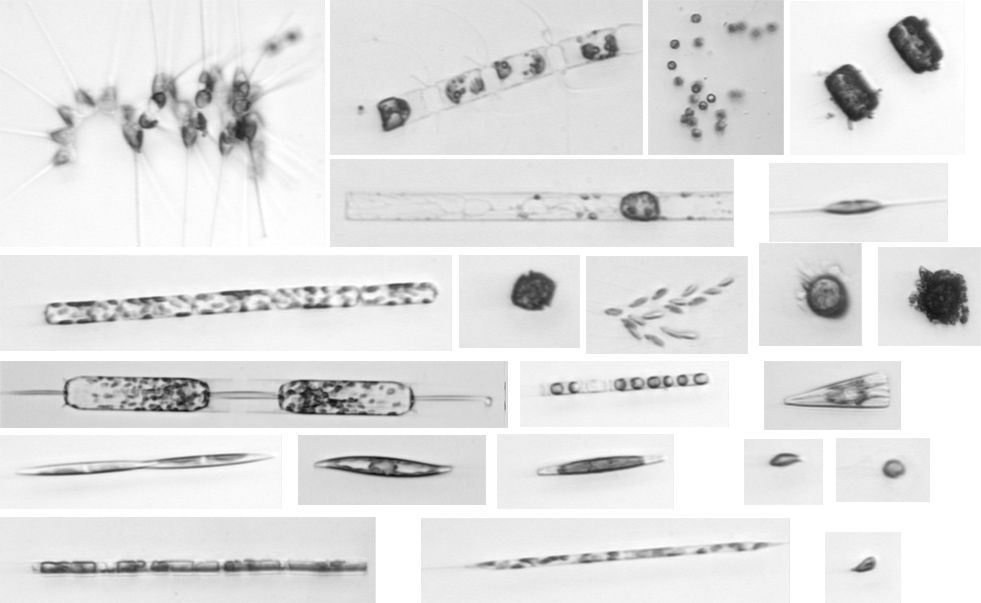
\includegraphics[height=5cm]{dataset/whoi/whoi}
  \caption{WHOI采集的数据集中每类浮游植物的例图}
  \label{fig:whoi}
\end{figure}

这22类图像中包含16类硅藻类图像:(1)星杆藻属(Asterionellopsis),(2)角毛藻属(Chaetoceros),(3)细柱藻属(Cylindrotheca),(4)指管藻属(Dactyliosolen),(5)DactFragCeratul,(6)双尾藻属(Ditylum),(7)几内亚藻属(Guinardia),(8)楔形藻属(Licmophora),(9)斜纹藻属(Pleurosigma),(10)拟菱形藻(Pseudonitzschia),(11)根管藻属(Rhizosolenia),(12)骨条藻属(Skeletonema),(13)海链藻属(Thalassiosira),(14)锥囊藻属(Dinobryon),(15)眼虫属(Euglena),(16)棕囊藻属(Phaeocystis)。除此之外还有4类由形态相似的浮游生物图像构成:(1)各种形状的纤毛虫(ciliate),(2)双鞭毛虫门(dinoflagellate),(3)鞭毛虫(nanoflagellate),(4)有翼的硅藻类(pennate diatoms)。另外还有两种海洋中的其他物质:一种是个体小于20$um$的不明物;另一种是碎石。整个数据集分为训练集和测试集,各包含3300张浮游植物图像,共6600张,其中每个类别中图像数量相等。

\subsection{ZooScan系统采集的数据集}
\label{sec:caldataset}

该数据集~\cite{gorsky2010digital}由ZooScan系统~\cite{grosjean2004enumeration}采集的浮游动物图像组成。数据集中包含20类浮游动物图像,其例图如图~\ref{fig:zooscan}所示。这20类图像中有14类为浮游动物:(1)螔螺属(Limacina),(2)翼足目(Pteropoda),(3)尖头溞属(Penilia),(4)长腹剑水蚤属(Oithona),(5)杯口水蚤目(Poecilostomatoida),(6)桡脚类亚纲(Copepoda)中的其他类生物,(7)十足目(Decapoda),(8)尾海鞘纲(Appendicularia),(9)樽海鞘纲(Thaliacae),(10)毛鄂动物门(Chaetognatha),(11)各类浮游生物的卵,(12)放射虫门(Radiolaria),(13)钟泳亚目(Calycophorae),(14)水母亚门(Medusae)。另外6类为非浮游生物:(1)气泡(bubble),(2)纤维(fiber),(3)聚集物(aggregates),(4)暗色聚集物(dark aggregates),(5)假浮游生物(pseudoplantkon),(6)采集到的聚焦不好的图像。该数据集共3771张图像,每类的图像数量各不相同,图~\ref{fig:zooscanNum}显示了数据集中每个类图像的数量,数量最少的类别有28张图像,最多的类别有427张。
\begin{figure}[H] % use float package if you want it here
  \centering
  \includegraphics[height=7cm]{dataset/zooscan/zooscan}
  \caption{ZooScan系统采集的数据集中每类浮游动物的例图}
  \label{fig:zooscan}
\end{figure}
\begin{figure}[H] % use float package if you want it here
  \centering
  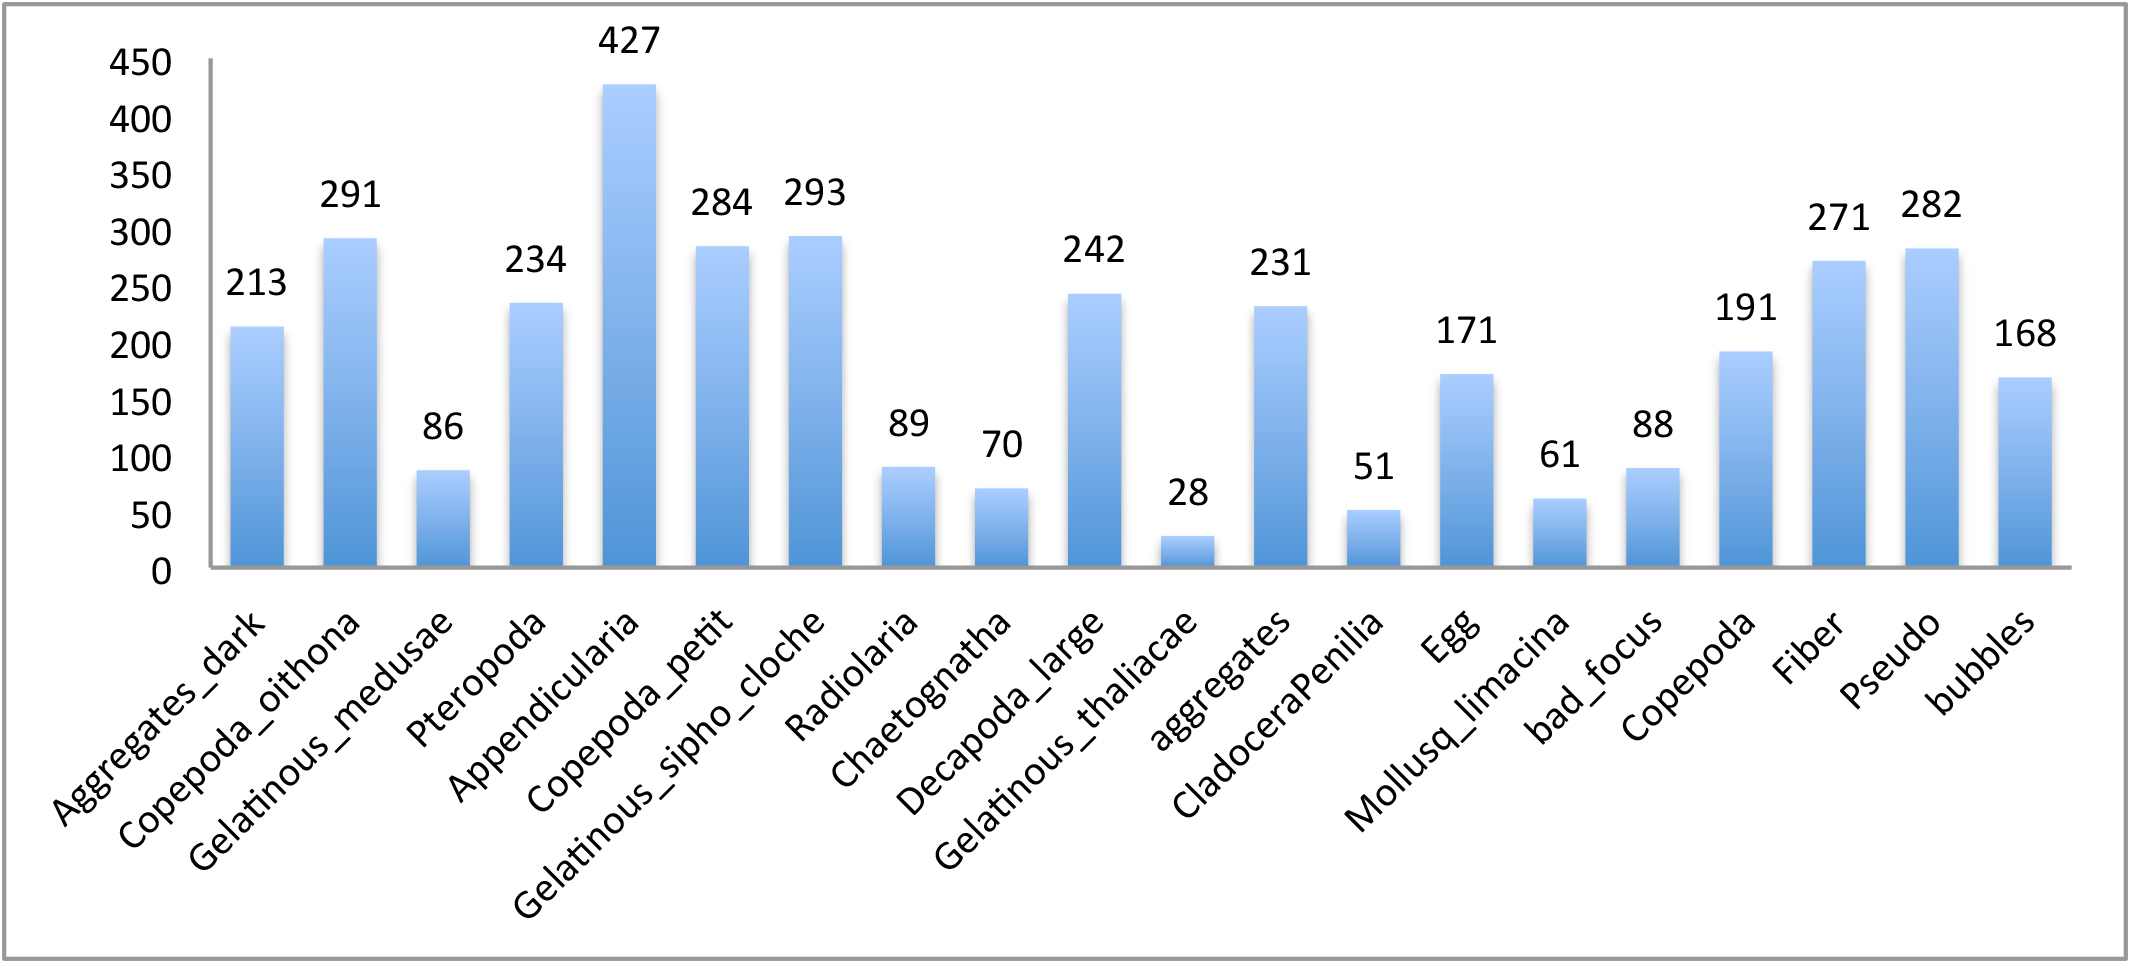
\includegraphics[height=5cm]{dataset/zooscan/zooscanNum}
  \caption{ZooScan系统采集的数据集中每类图像的数量}
  \label{fig:zooscanNum}
\end{figure}

%由于该数据集只有训练集,在用其进行实验时采用2折交叉验证的方法对分类器性能进行评价。

\subsection{Kaggle竞赛数据集}
\label{sec:kaggledataset}

Kaggle是一个数据分析的竞赛平台,研究者或企业可以将数据、问题发布在Kaggle平台上,通过竞赛的方式向大家征集解决方案。为了预测海洋健康程度,并为促进海洋健康做贡献,Kaggle竞赛平台上组织了浮游生物识别竞赛,根据浮游生物种群的丰富度衡量海洋生态系统的健康程度。Kaggle平台上的竞赛数据集由俄亥冈州立大学菲尔德海洋科学中心采集并提供,训练集共121类。本文实验中采用的数据集为该竞赛训练集的一部分,共选用38类浮游生物,例图如图~\ref{fig:kaggle}所示,其中35类为浮游生物,另外3类为非浮游生物。该数据集共28748张图像,每个类别数量各不相同,图~\ref{fig:kaggleNum}显示了每类图像的数量,数量最少的类别仅有108张图像,最多的有1979张图像。
\begin{figure}[H] % use float package if you want it here
  \centering
  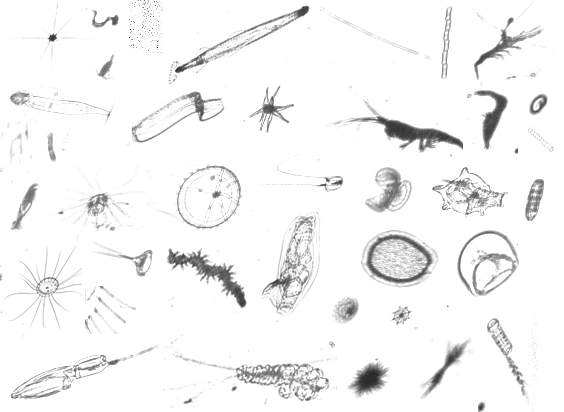
\includegraphics[height=7cm]{dataset/kaggle/kaggle}
  \caption{Kaggle竞赛数据集中每类浮游生物的例图}
  \label{fig:kaggle}
\end{figure}
\begin{figure}[H] % use float package if you want it here
  \centering
  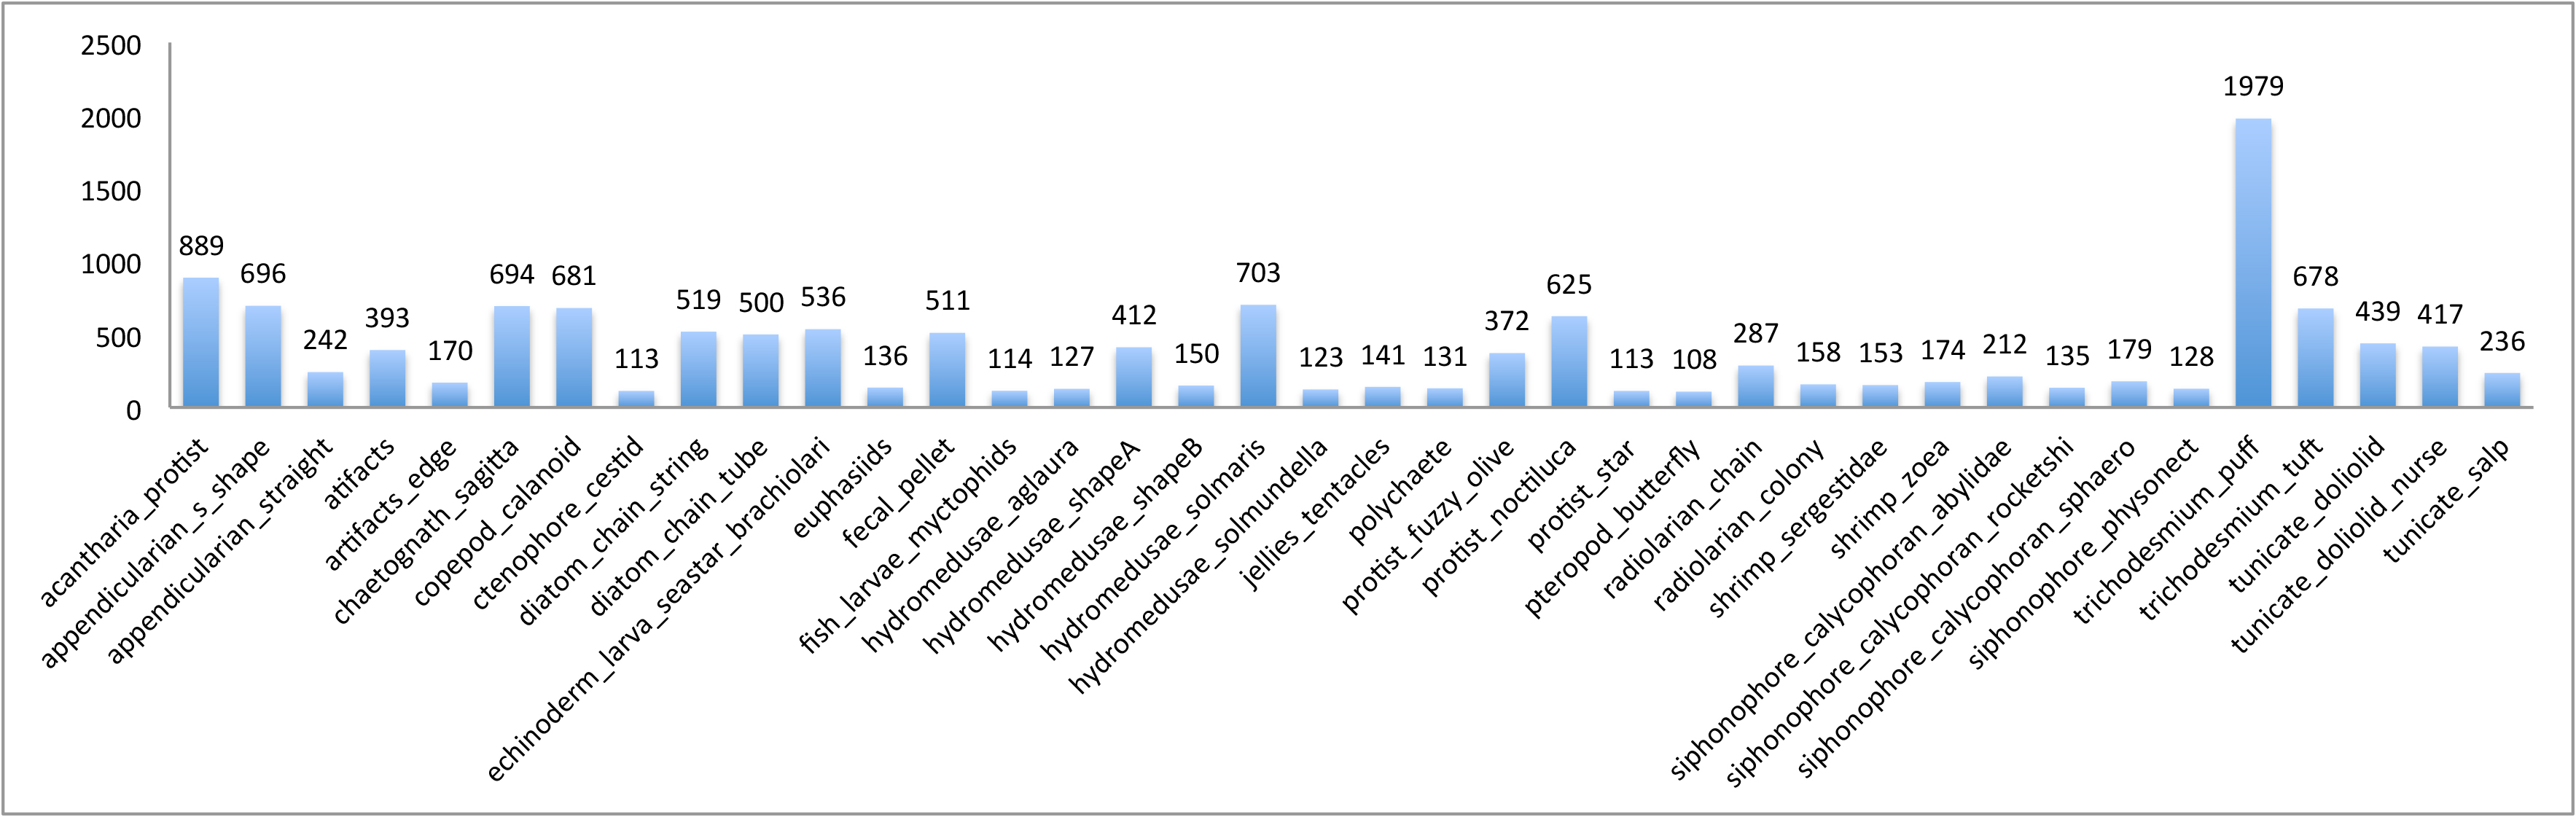
\includegraphics[height=5cm]{dataset/kaggle/kaggleNum}
  \caption{Kaggle竞赛数据集中每类图像的数量}
  \label{fig:kaggleNum}
\end{figure}


\section{浮游生物图像分类方法介绍}

目前对浮游生物图像分类的研究众多,下面分别介绍两种浮游生物图像分类系统:一个为浮游植物自动分类,由伍兹霍尔海洋研究所的Sosik等人提出;另一个是由法国国家科学院Gorsky等人研制的浮游动物图像扫描分析系统。这两个系统不仅具有较好的分类性能,而且被广泛应用于浮游生物分类,在后续实验中根据它们可以设计浮游生物分类系统性能的评价基准。

\subsection{伍兹霍尔海洋研究所浮游植物分类方法}

由于浮游生物个体小并且数量多,人工对其进行分类是不切实际的。伍兹霍尔海洋研究所的研究人员为了处理FlowCytobot采集的大量浮游植物图像,他们根据特征提取和模式识别算法提出一种浮游植物自动分类系统,该系统主要包括以下几个部分:

\begin{enumerate}
\item 图像预处理。在对图像中浮游植物形态特征进行提取时,除了需要目标的灰度纹理信息外,还需要用到目标的轮廓信息,因此要进行图像预处理,提取图像中目标生物的轮廓。在提取目标轮廓时,先采用相位一致性计算、边缘检测、数学形态学处理得到目标生物的二值图像,然后重新提取目标区域的简单边缘,从而可以获得图像中浮游生物的轮廓信息。
\item 特征提取。根据采集的原始浮游生物图像以及其对应的二值图像和轮廓边缘可以提取以下特征:简单的几何特征,例如目标的周长、长宽比、面积等;形状和对称性特征;纹理特征;不变矩;灰度共生矩阵等,共得到210个特征信息。这些特征主要通过MATLAB、DIPUM工具箱以及自定义函数生成。
\item 特征选择。由于采集的浮游生物特征中可能包含冗余或不相关的信息影响分类器的整体性能,因此采用特征选择去除冗余特征。
\item 训练分类器。特征选择后采用支持向量机来训练分类器,使用的核函数为高斯核函数(即径向基核函数),并采用10折交叉验证来确定核函数中的最优参数,该部分实验主要使用LIBSVM函数库实现。
\end{enumerate}

该分类方法在~\ref{sec:whoidataset}数据集上进行实验,使用训练集训练分类器,用获得的分类器对测试集图像进行分类,得到分类准确率可以达到88\%,其中有12个类别的分类结果超过了90\%,只有4类图像低于80\%。

\subsection{法国国家科学院浮游动物图像扫描分析系统}

浮游动物图像扫描分析系统(ZooScan Integrated System)是由法国国家科学院Villefranche海洋实验Gorsky等人发明的实验室浮游动物成像系统,该系统不仅可以完成对水下浮游动物从采集,而且能够对采集的图像进行识别~\cite{毕永坤2011基于}。与其他设备相比,ZooScan系统方便实用,并且具有较好的分类性能,目前该系统已经被广泛的商业化生产。

Zooscan系统由三部分组成,分别是Zooscan、ZooProcess和Plankton Identifier (PkID)。其中ZooScan为图像采集部分,将采集的浮游动物样本放在ZooScan仪器上,通过扫描形成数字图像。ZooProcess为软件部分,对ZooScan采集的浮游动物图像进行处理,分割提取并测量图像中的个体,可以自动得到图像中每个目标的参数,如灰度、大小、形状等参数。Plankton Identifier可以根据得到的参数对浮游生物图像进行分类。用ZooScan系统采集并识别浮游动物图像的过程如图~\ref{fig:zooscanframe}所示。
\begin{figure}[H] % use float package if you want it here
  \centering
  \includegraphics[height=8cm]{chart2/zooscan}
  \caption{ZooScan系统的基本流程}
  \label{fig:zooscanframe}
\end{figure}

使用ZooScan系统对采集的浮游动物进行分类时,首先用ZooProcess软件控制ZooScan扫描仪采集浮游动物图像:(1)扫描空白的背景图像;(2)扫描样本图像;(3)标准化原始图像;(4)用标准化得到的样本图像减去背景,并去除图像中的扫描框;(5)提取图像中的个体并测量每个个体的特征参数,测量得到的浮游生物特征参数共67个,大致可以分为四类:
\begin{enumerate}
\item 灰度参数,例如:
  \begin{itemize}
  \item Max,Min 物体灰度的最大、小值
  \item Mean 物体灰度的平均值
  \item IntDen 物体灰度值的总和
  \item StdDev 物体灰度值的标准差
  \end{itemize}
\item 大小参数,例如:
  \begin{itemize}
  \item Area 物体面积
  \item Perim 物体的周长
  \item Feret 物体的最大费雷特径
  \end{itemize}
\item 形状参数,例如:
  \begin{itemize}
  \item Fractal 物体的分形维数
  \item Circ 物体的圆形度
  \item Skelarea 物体骨架的像素数量
  \end{itemize}
\item 位置参数,例如:
  \begin{itemize}
  \item X,Y 物体的重心
  \item XM,YM 物体的灰度重心
  \item Height,Width 物体最小外接矩形的高和宽
  \end{itemize}
\end{enumerate}

然后,根据ZooProcess提取的特征参数,采用Plankton Identifier对采集的浮游动物图像进行分类:(1)构建训练集;(2)选用模式识别算法来训练分类器,PkID中提供的算法有K近邻、随机森林、C4.5、多层感知机、支持向量机(线性核函数、高斯核函数)等;(3)用训练得到分类器可以识别未知的浮游生物图像;(4)对预测结果进行人工校准。该分类系统在其采集的~\ref{sec:caldataset}数据集上的分类准确率可以达到78\%,分类效果最好的类别其准确率可以达到90\%以上。


\section{评价方法介绍}

评价一个分类系统性能主要从分类的准确度和可靠性两个方面进行,常用的评价方法有混淆矩阵、ROC曲线等,本文中采用的是混淆矩阵。

\subsection{混淆矩阵}

在机器学习领域,混淆矩阵(Confusion Matrix, CM)也被称为误差矩阵,是用来呈现算法性能的可视化工具,通常用于监督学习。若有n个类别,则混淆矩阵由n行n列组成,其中每一列表示每一类的预测样本数量,每一行表示每一类的实际样本数量,识别正确的样本数量为对角线,如表~\ref{tab:cm}所示。
\begin{table}[htbp]
  \centering
  \caption{混淆矩阵}
  \label{tab:cm}
  \begin{tabular}[c]{cccc}
    %\hline
    \toprule
    \multicolumn{2}{c}{\multirow{2}*{}} & \multicolumn{2}{c}{预测结果}\\
    %\cline{3-4}
    \multicolumn{2}{c}{} & 正样本 & 负样本\\
    %\hline
    \midrule
    \multirow{2}*{实际结果} & 正样本 & a & b\\
    %\cline{2-4}
     & 负样本 & c & d\\
    \bottomrule
    %\hline
  \end{tabular}
\end{table}

上表中a表示真阳性(True positives,TP),即正样本预测正确的数量;b表示正样本预测错误的样本数,即假阴性(False negatives,FN);c表示负样本被分为正样本的数目,即假阳性(False positives ,FP);d表示负样本预测正确的数量,即真阴性(True negatives ,TN)。根据这些数据可以计算出以下几个指标:
\begin{itemize}
\item 真阳性率(True positive rate,TPR),也是召回率(Recall),它表示正样本被正确识别的概率。
  \begin{eqnarray}
    TPR = \frac{a}{a+b}
  \end{eqnarray}
\item 假阳性率(False positive rate,FPR)表示负样本被误分为正样本的概率。
  \begin{eqnarray}
    FPR = \frac{c}{c+d}
  \end{eqnarray}
\item 真阴性率(True negative rate,TNR)表示负样本被正确分类的概率。
  \begin{eqnarray}
    TNR = \frac{d}{c+d}
  \end{eqnarray}
\item 假阴性率(False negative rate,FNR)表示正样本被误分为负样本的概率。
  \begin{eqnarray}
    FNR = \frac{b}{a+b}
  \end{eqnarray}
\item 错误发现率(False discovery rate,FDR)表示被预测为正样本中负样本的概率。
  \begin{eqnarray}
    FDR = \frac{c}{a+c}
  \end{eqnarray}
\item 阳性预测值(Positive predictive value,PPV),也称为命中率(Precision),表示在预测为正样本的样本中真正的正样本所占的比重。
  \begin{eqnarray}
    Precision = \frac{a}{a+c}
  \end{eqnarray}
\end{itemize}

本文实验中主要采用以下两个指标:Recall和Precision。由于Recall和Precision有时会出现矛盾情况,因此本文采用F-Measure评价分类器的性能。

%Recall越高,1-Precision越低,分类器的性能越好。

\subsection{F-Measure}

F-Measure是一种综合评价指标,也被称为F-Score,当Recall和Precision出现矛盾时,就可以采用该方法进行评价。
\begin{eqnarray}
F=\frac{(\alpha^{2}+1)P*R}{\alpha^{2}(P+R)}
\end{eqnarray}
其中$\alpha$为参数,$P$代表Precision,$R$为Recall。

当$\alpha=1$就得到F1-Measure:
\begin{eqnarray}
F1=\frac{2*PR}{P+R}
\end{eqnarray}

F1的值较高说明试验分类模型性能更好。

\subsection{交叉验证}

交叉验证(Cross Validation)是一种检验分类器性能的方法,该方法将数据集分为训练集和验证集,首先用训练集训练分类器,然后用获得的分类器对验证集进行识别,其分类结果为评价分类器性能的指标\cite{王怀亮2011交叉验证在数据建模模型选择中的应用}。在评价过程中使用交叉验证可以得到更加稳定可靠的评价结果。常用的交叉验证形式有:Hold-out验证、K折交叉验证(K-fold Cross Validation,K-CV)、留一验证(Leave-One-Out Cross Validation,LOO-CV)。
\begin{itemize}
\item Hold-out验证是将数据集划分为两集合:一个作为训练集,用其训练分类器;另一个作为验证集,用其对分类器进行测试,最终得到的分类结果可以作为该分类器的性能指标。
\item K折交叉验证就是将数据集划分为K个子集,将每一个子集分别看做验证集进行实验,与此同时另外K-1个部分作为训练集。一共要进行K次实验,训练获得K个分类模型,每个模型对验证集进行分类会得到一个准确率,这K个准确率的平均值可以作为该分类器评价指标。
\item 留一验证的基本思想为:若原数据集一共n个样本,则将每个样本单独看做验证集,另外n-1个组成训练集。与K折交叉验证类似,留意验证一共需要进行n次实验,获得n个训练模型和分类准确率,计算n个准确率的平均值可以作为分类器的评价指标。
\end{itemize}

本文对分类器性能进行评价时采用K折交叉验证。

\section{本章小结}

在介绍基于多核学习的浮游生物分类研究之前,本章先介绍了浮游生物分类的相关背景。首先介绍的是浮游生物的相关内容;然后详细介绍后续实验中所用的数据集;接下来介绍目前分类性能较好的浮游生物分类方法,在后面的实验里将根据它们设计对比实验的基准;在本章最后介绍了对分类系统性能进行评价的方法,本文使用了K折交叉验和混淆矩阵来统计得到的分类结果,从而对分类器性能进行评价。





